% AUTHOR: AIMEN ZELACI
% DATE: 04/17/2020
\documentclass[12pt]{IEEEtran}

\linespread{1.5}
\usepackage{color,soul}
\usepackage{tikz}
\usetikzlibrary{shapes.geometric, arrows, shapes.arrows, decorations.markings, calc}
\usepackage{pgfplots}

\usepackage[english]{babel}
\usepackage{graphicx}
\usepackage{subcaption}
\usepackage{hyperref}
\usepackage{cite}


\tikzstyle{data} = [
	cylinder, 
	shape border rotate=90, 
	draw,
	minimum width=1.5cm, 
	minimum height=1.2cm,
	text centered, 
	draw=black, 
	line width=0.3mm,
	shape aspect=.1
]
\tikzstyle{testing} = [
	thick,
	<->,
]

\tikzstyle{forward} = [
	thick,
	->,
]


\tikzstyle{operation} = [
	rectangle, 
	rounded corners,
	minimum width=2cm, 
	minimum height=1.2cm,
	text centered, 
	draw=black, 
	line width=0.6mm,
]

\tikzstyle{segment} = [
	rectangle, 
	rounded corners,
	minimum width=1cm, 
	minimum height=0.5cm,
	text centered, 
	draw=black, 
	line width=0.6mm,
]

\tikzstyle{header} = [
	rectangle, 
	rounded corners,
	minimum width=1.3cm, 
	minimum height=0.5cm,
	text centered, 
	draw=black, 
	line width=0.6mm,
]


\begin{document}

\title{\hl{The concept of layering in the context of sending an e-mail message}}

\author{Aimen Zelaci}

\maketitle

\begin{document}
\section{Discussion}
The journey of the E-mail message sets sail from the sender's (host A) operating system. The first layer it encounters is the application layer. This layer is a software built on top of a protocol. If the E-mail at hand is a web mail, the application layer would the web browser and the corresponding protocol is HTTP (Hyper Text Transfer Protocol). However, if the user is using an E-mail GUI, the most common protocol is SMTP (Simple Mail Transfer Protocol). This layer acts as an interface to the network.
Now that we know how to face the network, we need to encode, encrypt and compress the message. Text will be encoded using ASCII (American Standard Code for Information Interchange) and other types of data will encoded into their corresponding formats, such as JPEG for images. To encrypt the data, SSL (Secret Socket Layer) scheme is the most widely used. The third main role of this layer is compressing the data: to shorten the information for efficient transmission.
Host A might run several applications on his operating system, therefore a session is needed for each different connection, to synchronize, control dialogue, manage tokens and establish a recovery setup. This is where the Session layer comes into play. 
In order to grasp the next stage, we must point out under which cover this whole operation is running, it is called the Client-server model (still an E-mail can be sent via peer-to-peer, but that is beyond the scope of this discussion). In this model a client sends a request to a specific computer, called a server, and that server will act accordingly to provide the service. In this case host A will be our client and the server will be some E-mail server. When the E-mail reaches the server, the latter needs to identify what service host A exactly requested. In order to accomplish that, the transport layer at this stage attaches a header to our E-mail, this header contains the destination port as well as the source port that allow the server to provide the correct service. Before that transport layer dissects the E-mail into different segments to ensure reliability or efficiency. The transport layer incorporates different protocols that the designer must specify for the communication process. For E-mail most organizations use the TCP (Transmission Control Protocol), to achieve same order delivery and develops processes to control the flow of data, in other words this layer decides how many segments to send so that the receiver is not over whelmed. To finalise this stage, we are going to investigate a bit further the header that the transport layer attaches to the segments. In addition to the destination port and source port, this header contains sequence numbers which defines the parts of the data. Also, it contains acknowledgement numbers which in turn allow the server to know what it has received or what it is going to receive next acknowledging what already came in.  
Segments will then be sent through multiple paths to reach their destination, by the means of a router. The layer responsible for this process is the networking layer. This layer adds another header to the segment, to be then upgraded into a packet. This header deploys an addressing mechanism to identify end devices i.e the sender and the receiver. The most common addressing scheme is the IP addressing.
At this point our E-mail data is streams of bits and must be linked somehow to the physical layer. The data link layer does so by dividing the data into data frames. The frame is built by attaching to the packet a trailer and a header. The header and trailer carry the information to the physical layer about when the frame begins and when it ends. The data link layer consists of two sublayers: Logical layer and a MAC layer (Medium Access Layer), and they are both used to link the physical part to the logical through physical addressing. Furthermore, this layer performs error handling by employing different mechanisms such as the checksum that is attached to the data before it is sent. I employed a Python program to intercept messages in a local network and show the amount of frames in the exchanges, as shown in figure 2.
\begin{figure}
  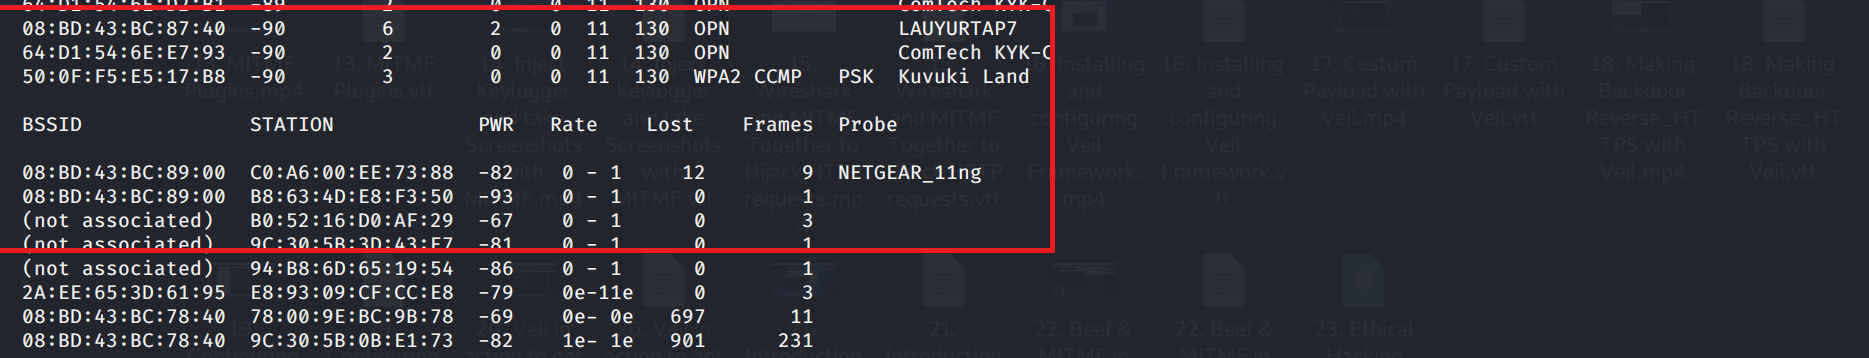
\includegraphics[width=\linewidth]{data_frame.png}
  \caption{BSSID: the address of the network. Station: MAC address of the client. Frames: amount of data frames exchanged}
  \label{fig:Data frames}
\end{figure}
Finally, the E-mail has reached the physical layer. This layer includes different types of wires and transmission mediums, for example, coaxial, twisted pair and fiber-optic cables. Next, the data at is sent via the physical medium, at host B the reverse operation will occur and the E-mail will build its way up to the application layer of host B, removing the headers at each stage accordingly. Figure 1 demonstrates the entire process of sending an E-mail message under the OSI seven layers model.

\begin{figure}[h]
        \resizebox{10cm}{8cm}{%
	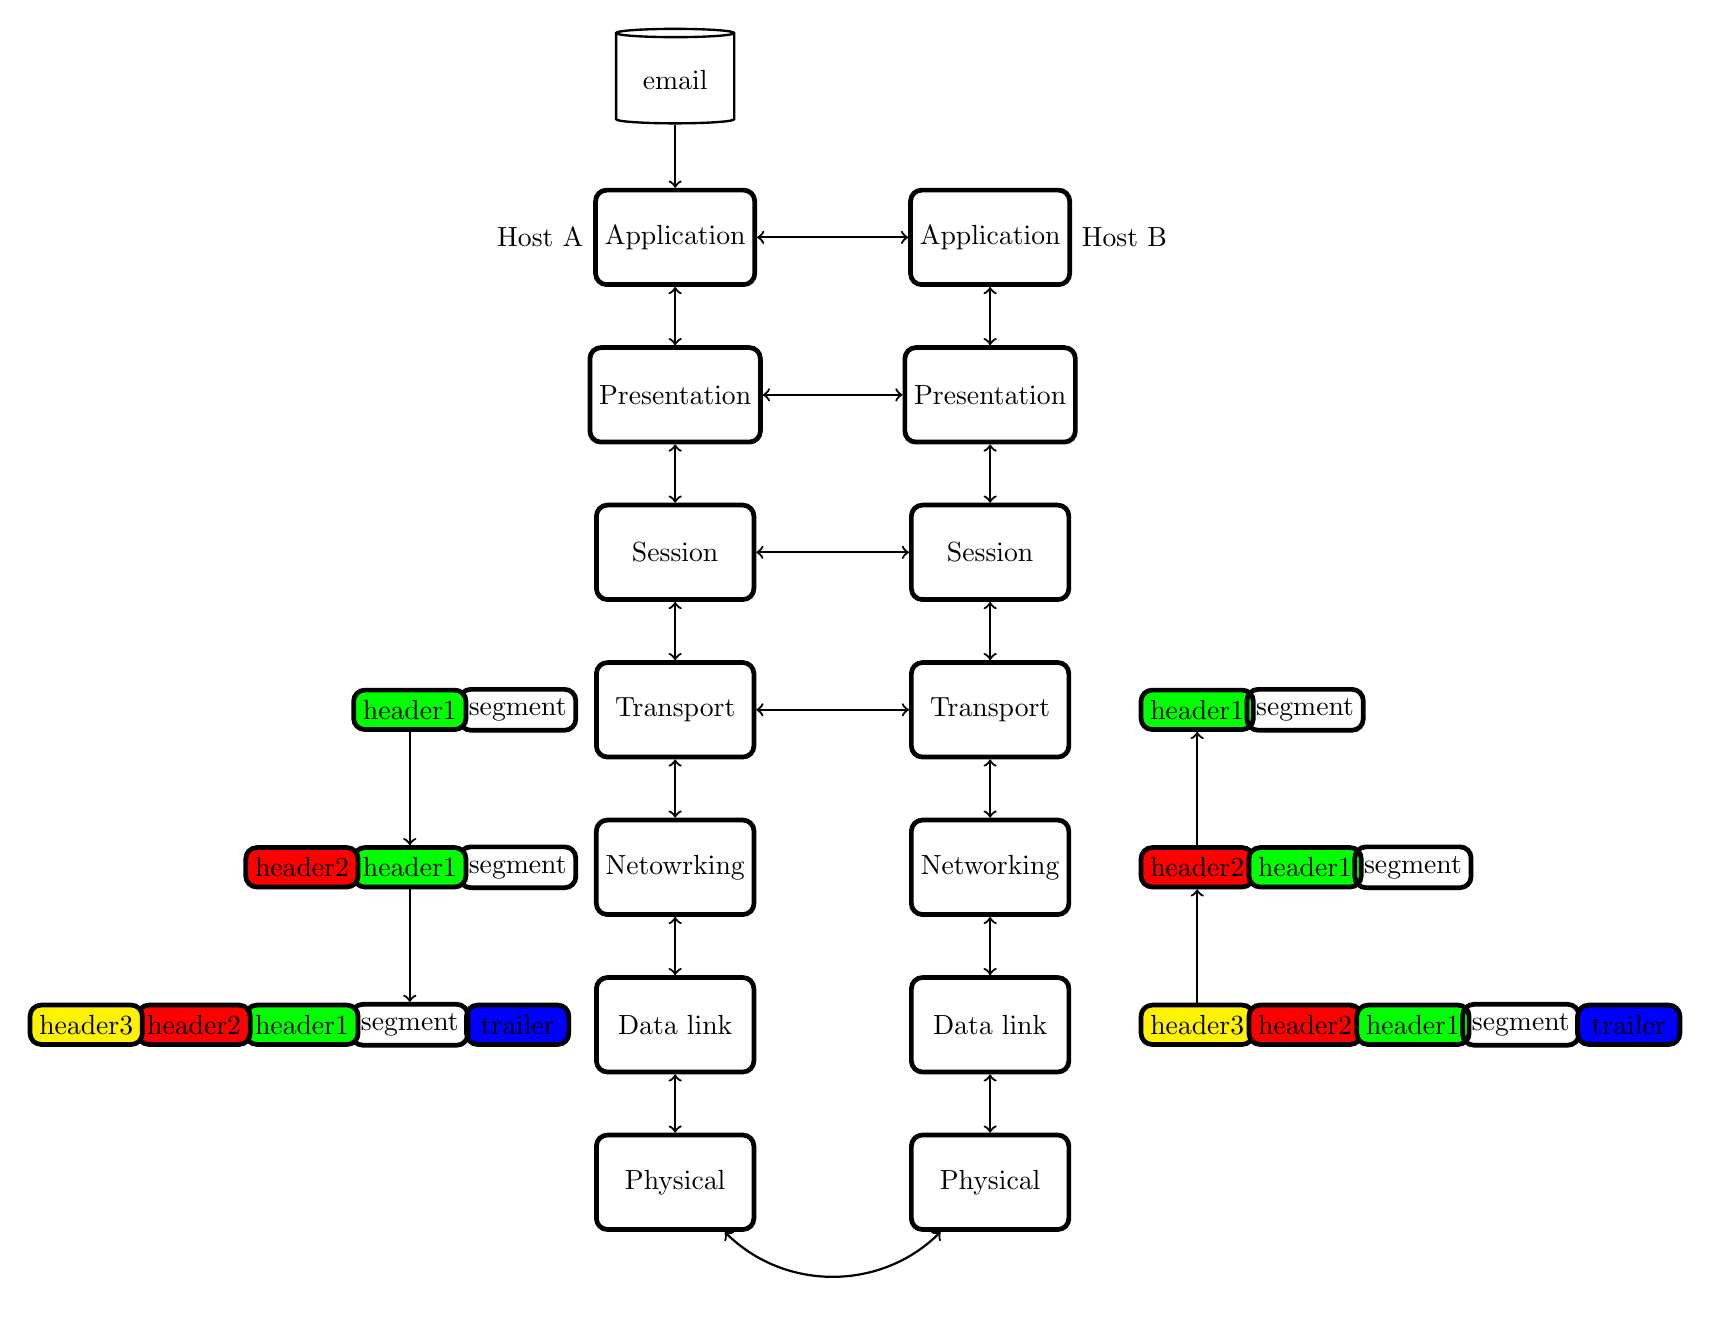
\begin{tikzpicture}[node distance=2cm]
\node (email) [data]{email};
\node (layer1A) [operation, below of=email, label=left:Host A] {Application};
\node (layer2A) [operation,below of=layer1A] {Presentation};
\node (layer3A) [operation,below of=layer2A] {Session};
\node (layer4A) [operation,below of=layer3A] {Transport};

\node (segment)[segment, left of=layer4A]{segment};
\node (header)[header, fill=green,left of=segment, xshift=0.63cm]{header1};

\node (layer5A) [operation,below of=layer4A] {Netowrking};

\node (segment)[segment, left of=layer5A]{segment};
\node (header1)[header,fill=green, left of=segment, xshift=0.63cm]{header1};
\node (header2)[header, fill=red,left of=header1, xshift=0.63cm]{header2};

\node (layer6A) [operation,below of=layer5A] {Data link};
\node (trailer)[header, fill=blue,left of=layer6A]{trailer};
\node (segment)[segment, left of=trailer, xshift=0.63cm]{segment};
\node (header16)[header, fill=green,left of=segment, xshift=0.63cm]{header1};
\node (header26)[header, fill=red,left of=header16, xshift=0.63cm]{header2};
\node (header36)[header, fill=yellow,left of=header26, xshift=0.63cm]{header3};
\node (layer7A) [operation,below of=layer6A] {Physical};

\draw [forward] (email) -- (layer1A);
\draw [forward] (header) -- (header1);
\draw [forward] (header1) -- (segment);
\draw [testing] (layer1A) -- (layer2A);
\draw [testing] (layer2A) -- (layer3A);
\draw [testing] (layer3A) -- (layer4A);
\draw [testing] (layer4A) -- (layer5A);
\draw [testing] (layer5A) -- (layer6A);
\draw [testing] (layer6A) -- (layer7A);


\node (layer1B) [operation, right of=layer7A, xshift=2cm] {Physical};
\draw [testing] (layer7A) to [bend right=45] (layer1B);

\node (layer2B) [operation,right of=layer6A, xshift=2cm] {Data link};



\node (header3B)[header, fill=yellow,right of=layer2B, xshift=0.63cm]{header3};
\node (header2B)[header, fill=red,right of=header3B, xshift=-0.63cm]{header2};
\node (header1B)[header, fill=green,right of=header2B, xshift=-0.63cm]{header1};
\node (segmentB)[segment, right of=header1B, xshift=-0.63cm]{segment};
\node (trailerB)[header, right of=segmentB, fill=blue,xshift=-0.63cm]{trailer};

\node (layer3B) [operation, right of=layer5A, xshift=2cm] {Networking};

\node (header22B)[header, fill=red,right of=layer3B, xshift=0.63cm]{header2};
\node (header12B)[header, fill=green,right of=header22B, xshift=-0.63cm]{header1};
\node (segmentB)[segment, right of=header12B, xshift=-0.63cm]{segment};

\node (layer4B) [operation, right of=layer4A, xshift=2cm] {Transport};

\node (header13B)[header, fill=green,right of=layer4B, xshift=0.63cm]{header1};
\node (segmentB)[segment, right of=header13B, xshift=-0.63cm]{segment};

\node (layer5B) [operation, right of=layer3A, xshift=2cm] {Session};
\node (layer6B) [operation, right of=layer2A, xshift=2cm] {Presentation};
\node (layer7B) [operation, right of=layer1A, xshift=2cm, label=right:Host B] {Application};


\draw [forward] (header3B) -- (header22B);
\draw [forward] (header22B) -- (header13B);

\draw [testing] (layer4B) -- (layer4A);
\draw [testing] (layer5B) -- (layer3A);
\draw [testing] (layer6B) -- (layer2A);
\draw [testing] (layer7B) -- (layer1A);

\draw [testing] (layer1B) -- (layer2B);
\draw [testing] (layer2B) -- (layer3B);
\draw [testing] (layer3B) -- (layer4B);
\draw [testing] (layer4B) -- (layer5B);
\draw [testing] (layer5B) -- (layer6B);
\draw [testing] (layer6B) -- (layer7B);
	\end{tikzpicture}
}
	\caption{Sending an E-mail from host A to host B in the context of OSI 7 layer reference model}
	\label{fig:overall}
	
\end{figure}


\end{document}